For the computational experiments a batch of tests was driven to find the best
parameters for the problem using the well-known set of problems defined by two sets:
a first set composed by 270 instances provided by Chu and Beasley (\cite{Chu-Beasley-1998})
and a second set composed by 11 instances provided by Glover and Kochenberger in
\cite{glover1996critical}.
These instances are all available at \cite{ORLibrary}.
%Afterwards two main tests was considered:
%(a) using the well-known set of problems defined by Chu and Beasley (\cite{Chu-Beasley-1998})
%and (b) a large set of randomly generated instances using uniform distribution.

The set of MKP instances provided by Chu and Beasley was generated using a
procedure suggested by Freville and Plateau~\cite{freville1994efficient}, which
attempts to generate instances hard to solve.
The number of constraints $m$ varies among $5$, $10$ and $30$, and the number
of variables $n$ varies among $100$, $250$ and $500$.

The $w_{ij}$ were integer numbers drawn from the discrete uniform distribution
$U(0, 1000)$.
The capacity coefficient $c_i$ were set using
$b_i = \alpha\sum_{j=1}^{n} w_{ij}$ where $\alpha$ is a tightness ratio and
varies among $0.25$, $0.5$ and $0.75$.
For each combination of $(m,n,\alpha)$ parameters, $10$ random problems was generated,
totaling $270$ problems.
The profit $p_j$ of the items were correlated to $w_{ij}$ and generated as follows:
\begin{displaymath}
  p_j = \sum_{i=1}^m \frac{w_{ij}}{m} + 500q_j \qquad j = 1, \ldots, n
\end{displaymath}

%\subsection{The set of random instances}

%The second set of instances is composed by problems generated using a similar
%setup.
%The only differences is that the profit $p_j$ is also drawn from a discrete uniform
%distribution $U(0, 1000)$.
%For each combination of $(m, n, \alpha)$ parameter, $600$ random problems was
%generated, totaling $16200$ problems.

\subsection{Experimental results}

All the experiments were run on a Intel$^R$ Core i5-3570 CPU @3.40GHz computer
with 4GB of RAM.
The SCE algorithm for MKP was implemented in C programming language.
%For the set of random instance all best known solution was found by the solver
%SCIP 3.0.1 running for at least 10 minutes.

For the variable fixing procedure, the range size of the approximate core was
$|C| = m+\frac{n}{10}$ for all instances.
After a previous batch test the following parameters for SCE were defined and used
in all executions of SCE:
\begin{itemize}
  \item $N = 20$: number of complexes;
  \item $M = 20$: number of individuals in each complex;
  \item $P = 5$: number of individuals in each subcomplex;
  \item $K = 300$: number of algorithm iterations;
  \item $K' = 20$: number of iterations used in the complex evolving process;
  \item $c = n/5$: number of genes carried from parent in crossing process.
\end{itemize}

Table~\ref{tab:chu} shows the performance of the SCE on the Chu-Beasley set of instances.
Each instance in the set was executed 10 times on SCE.
Columns \textit{n}, \textit{m} and \textit{$\alpha$} shows the parameters used
on each instance generation.
The \textit{SCE time} column shows the average execution time of SCE algorithm.
The \textit{quality} column shows the average ratio of the solution found by SCE and
the best known solution from literature of each instance (\cite{vimont2008reduced, della2012improved}).
It can be observed that the SCE has a fast convergence speed, achieving high
quality solutions, at least $99.02\%$ of best known, in less than $2$ seconds
for every instance.

\begin{table}
{
\renewcommand{\arraystretch}{1.5}%
\fontsize{8.5pt}{1em}\selectfont 
\begin{center}
\begin{tabular}{|r|r|r|rr|} \hline
\textbf{n}   & \textbf{m}  & \textbf{$\alpha$} & \textbf{SCE time (s)} & \textbf{quality (\%)} \\ \hline
100 &  5 & 0.25 & 0.15 & 99.73 \\
    &    & 0.50 & 0.15 & 99.86 \\
    &    & 0.75 & 0.13 & 99.91 \\ \cline{2-5}
    & 10 & 0.25 & 0.22 & 99.53 \\
    &    & 0.50 & 0.22 & 99.76 \\
    &    & 0.75 & 0.22 & 99.96 \\ \cline{2-5}
    & 30 & 0.25 & 1.00 & 99.02 \\
    &    & 0.50 & 0.79 & 99.21 \\
    &    & 0.75 & 0.77 & 99.52 \\ \cline{2-5}
    & \multicolumn{3}{r}{\textbf{average quality}}  & $\bf 99.50$  \\ \hline \hline
\textbf{n}   & \textbf{m}  & \textbf{$\alpha$} & \textbf{SCE time (s)} & \textbf{quality (\%)} \\ \hline
250 &  5 & 0.25 & 0.54 & 99.87 \\
    &    & 0.50 & 0.55 & 99.94 \\
    &    & 0.75 & 0.51 & 99.95 \\ \cline{2-5}
    & 10 & 0.25 & 0.67 & 99.57 \\
    &    & 0.50 & 0.62 & 99.80 \\
    &    & 0.75 & 0.64 & 99.88 \\ \cline{2-5}
    & 30 & 0.25 & 1.16 & 99.46 \\
    &    & 0.50 & 0.96 & 99.36 \\
    &    & 0.75 & 1.03 & 99.59 \\ \cline{2-5}
    & \multicolumn{3}{r}{\textbf{average quality}}  & $\bf 99.60$  \\ \hline \hline
\textbf{n}   & \textbf{m}  & \textbf{$\alpha$} & \textbf{SCE time (s)} & \textbf{quality (\%)} \\ \hline
500 &  5 & 0.25 & 0.85 & 99.77 \\
    &    & 0.50 & 0.86 & 99.87 \\
    &    & 0.75 & 0.84 & 99.92 \\ \cline{2-5}
    & 10 & 0.25 & 0.99 & 99.49 \\
    &    & 0.50 & 0.97 & 99.78 \\
    &    & 0.75 & 0.95 & 99.83 \\ \cline{2-5}
    & 30 & 0.25 & 1.53 & 99.75 \\
    &    & 0.50 & 1.48 & 99.42 \\
    &    & 0.75 & 1.42 & 99.68 \\ \cline{2-5}
    & \multicolumn{3}{r}{\textbf{average quality}}  & $\bf 99.61$  \\ \hline
\end{tabular}
\end{center}
}
 \caption{SCE performance on Chu-Beasley problems.}
 \label{tab:chu}
\end{table}

Table~\ref{tab:gk} shows the performance of the SCE on the Glover-Kochenberger set of instances.
Each instance in the set was executed 10 times on SCE.
Columns \textit{n} and \textit{m} indicate the size of each instance.
The \textit{SCE time} column shows the average execution time of SCE algorithm.
The \textit{quality} column shows the average ratio of the solution found by SCE and
the best known solution of each instance.
It can be noticed that SCE achieved high quality solutions, at least $99.10\%$
of best known solution, spending very small amount of processing time.

\begin{table}
{
\renewcommand{\arraystretch}{1.5}%
\fontsize{8.5pt}{1em}\selectfont 
\begin{center}
\begin{tabular}{|r|r|r|r|r|} \hline
		\textbf{\#} & \textbf{n}   & \textbf{m}  & \textbf{SCE time (s)} & \textbf{quality (\%)} \\ \hline
01 & 100 & 15 & 0.31 & 99.68 \\ \hline
02 & 100 & 25 & 0.47 & 99.51 \\ \hline
03 & 150 & 25 & 0.79 & 99.60 \\ \hline
04 & 150 & 50 & 1.61 & 99.10 \\ \hline
05 & 200 & 25 & 0.83 & 99.73 \\ \hline
06 & 200 & 50 & 1.67 & 99.30 \\ \hline
07 & 500 & 25 & 1.27 & 99.72 \\ \hline
08 & 500 & 50 & 2.06 & 99.62 \\ \hline
09 &1500 & 25 & 1.83 & 99.32 \\ \hline
10 &1500 & 50 & 5.25 & 99.76 \\ \hline
11 &2500 &100 &11.94 & 99.77 \\ \cline{1-5}
    \multicolumn{4}{|r|}{\textbf{average quality}}  & $\bf 99.46$  \\ \hline
\end{tabular}
\end{center}
}
 \caption{SCE performance on Glover-Kochenberger problems.}
 \label{tab:gk}
\end{table}

%\begin{table}
%{
%\renewcommand{\arraystretch}{1.5}%
%\fontsize{8.5pt}{1em}\selectfont 
%\begin{center}
%\begin{tabular}[c]{|r|r|r|rrr|} \hline
%\textbf{n}   & \textbf{m}  & \textbf{$\alpha$}    &\textbf{SCIP time (s)}& \textbf{SCE time (s)} & \textbf{gap (\%)} \\ \hline
%100 &  5 & 0.25 & $  0.93$ & $  0.41$  & $98.3$ \\
%    &    & 0.50 & $  0.28$ & $  0.39$  & $99.3$ \\
%    &    & 0.75 & $  0.09$ & $  0.37$  & $99.8$ \\ \cline{2-6}
%    & 10 & 0.25 & $  3.15$ & $  0.41$  & $98.2$ \\
%    &    & 0.50 & $  0.71$ & $  0.40$  & $99.3$ \\
%    &    & 0.75 & $  0.16$ & $  0.37$  & $99.8$ \\ \cline{2-6}
%    & 30 & 0.25 & $  7.26$ & $  0.42$  & $98.3$ \\
%    &    & 0.50 & $  1.47$ & $  0.42$  & $99.3$ \\
%    &    & 0.75 & $  0.25$ & $  0.38$  & $99.8$ \\ \cline{2-6}
%    & \multicolumn{4}{r}{\textbf{average gap}}  & $\bf 99.1$  \\ \hline \hline
%\textbf{n}   & \textbf{m}  & \textbf{$\alpha$}    &\textbf{SCIP time (s)}& \textbf{SCE time (s)} & \textbf{gap (\%)} \\ \hline
%250 &  5 & 0.25 & $ 58.20$ & $  1.10$  & $97.2$ \\
%    &    & 0.50 & $  8.51$ & $  1.04$  & $98.9$ \\
%    &    & 0.75 & $  0.51$ & $  0.90$  & $99.7$ \\ \cline{2-6}
%    & 10 & 0.25 & $227.94$ & $  1.11$  & $97.6$ \\
%    &    & 0.50 & $ 43.69$ & $  1.02$  & $99.0$ \\
%    &    & 0.75 & $  1.59$ & $  0.90$  & $99.8$ \\ \cline{2-6}
%    & 30 & 0.25 & $270.48$ & $  1.20$  & $97.7$ \\
%    &    & 0.50 & $ 88.73$ & $  1.09$  & $99.0$ \\
%    &    & 0.75 & $  2.90$ & $  0.94$  & $99.8$ \\ \cline{2-6}
%    & \multicolumn{4}{r}{\textbf{average gap}}  & $\bf 98.7$  \\ \hline \hline
%\textbf{n}   & \textbf{m}  & \textbf{$\alpha$}    &\textbf{SCIP time (s)}& \textbf{SCE time (s)} & \textbf{gap (\%)} \\ \hline
%500 &  5 & 0.25 & $278.85$ & $  2.23$  & $96.1$ \\
%    &    & 0.50 & $177.32$ & $  2.14$  & $98.4$ \\
%    &    & 0.75 & $  8.47$ & $  1.87$  & $99.6$ \\ \cline{2-6}
%    & 10 & 0.25 & $284.11$ & $  2.30$  & $96.7$ \\
%    &    & 0.50 & $275.68$ & $  2.16$  & $98.6$ \\
%    &    & 0.75 & $ 33.67$ & $  1.90$  & $99.7$ \\ \cline{2-6}
%    & 30 & 0.25 & $283.78$ & $  2.50$  & $96.9$ \\
%    &    & 0.50 & $283.54$ & $  2.32$  & $98.7$ \\
%    &    & 0.75 & $ 71.66$ & $  1.96$  & $99.7$ \\ \cline{2-6}
%    & \multicolumn{4}{r}{\textbf{average gap}}  & $\bf 98.3$  \\ \hline
%\end{tabular}
%\end{center}
%}
% \caption{SCE performance on the random generated problems.}
% \label{tab:rand}
%\end{table}

%\begin{figure}
%  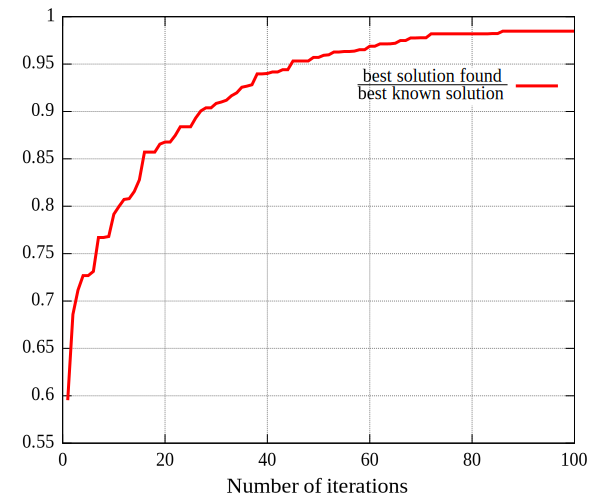
\includegraphics[scale=0.5]{imgs/iter}
%  \caption{Convergence process of SCE for MKP
%    for a problem with $n=500$, $m=30$ and $t=0.50$.}
%  \label{fig:iter}
%\end{figure}

%The fast convergence speed of SCE for MKP can be noticed in Fig.~\ref{fig:iter}.
%The figure shows for each iterations step, the quality of best solution found
%for the first $100$ iterations.
%The problem instance used was taken from the second set of problem (random instances).
%The best known solution was found with $600$s of execution on SCIP solver and
%the execution of the SCE algorithm expended $1.1$ seconds.
